\documentclass[12pt,a4paper,norsk]{article}
\usepackage[utf8]{inputenc}
\usepackage[norsk]{babel}
\usepackage{hyperref} % for hyperlenker mellom ref og label
\usepackage{amsmath}
\usepackage{amssymb}
\usepackage{amstext} % for \text macro
\usepackage{array}   % for \newcolumntype macro
\newcolumntype{C}{>{$}c<{$}} % math-mode version of "l" column type
\usepackage[dvipsnames]{xcolor} % Farger :)
\usepackage{siunitx}
\usepackage{subcaption} %for subfigure
\usepackage{float}
\usepackage{booktabs} %for nice table lines
\usepackage[siunitx, american, europeanresistors, RPvoltages]{circuitikz} % for kretser
\usepackage{graphicx} % for bilder
\graphicspath{{./}}

\usepackage[skip=5mm]{parskip} % mellom mellom paragrafer, ikke indent
\usepackage{caption} % For å putte caption på figurer i minipage
\usepackage{tikz-timing} % For rising og falling edge
\usepackage{randtext} % Enkel e-post-obfuskering

\newcommand{\resi}[1]{\frac{1}{#1}}
\newcommand{\red}[1]{{\color{Red}#1}}
\newcommand{\green}[1]{{\color{ForestGreen}#1}}
\newcommand{\blue}[1]{{\color{MidnightBlue}#1}}
\newcommand{\orange}[1]{{\color{Orange}#1}}
\newcommand{\purple}[1]{{\color{Plum}#1}}
\newcommand{\brown}[1]{{\color{Sepia}#1}}
\newcommand{\maroon}[1]{{\color{Maroon}#1}}
\newcommand{\rising}{\texttiming{[-,timing/slope=0]LH}}
\newcommand{\falling}{\texttiming{[-,timing/slope=0]HL}}

\title{TFE4101 Krets- og Digitalteknikk}
\newcommand{\lst}{krogstie}
\newcommand{\fst}{havard}
\author{Håvard Krogstie\\\randomize{\lst{}.\fst{}@gmail.com}}
\date{\today}

\begin{document}

\maketitle

\noindent
Dette dokumentet inneholder forklaringer, definisjoner, metoder og formler brukt
i TFE4101 Krets- og Digitalteknikk ved NTNU våren 2020 (Den med Corona). Det er
en personlig gjennomgang av det som virket relevant, og utfyllende nok til at jeg
ikke skal trenge noe annet på hjemmeeksamen. Dokumentet inneholder kretsteori,
metoder for regning på kretser, teorien bak kondensatorer og spoler, dioder,
transistorer, CMOS, logiske kretser, boolsk algebra, binærtallsregning, timing
av digitale kretser og sekvensielle kretser. Seksjonene blir mer utfyllende
underveis.

Dokumentet har gjevnt over ikke kildehenvisninger, og er ikke vurdert av noen
med kunnskap i faget. Du finner heller ikke øvingskok her. Les på eget ansvar.
Kildekode og nyeste utgave på
\href{https://github.com/haved/notater/}{github.com/haved/notater}. Skrivefeil,
faktafeil, mangler eller uklaheter? Opprett en issue eller skriv en e-post!

\clearpage
\tableofcontents
\clearpage

\section{Kretser}
Kretser er samlinger med komponenter koblet sammen. Kretsen kan modeleres som en
graf der koblinger er noder, og komponentene blir kanter mellom
nodene. Ofte ser vi ikke på ledninger som komponenter, men bare som
ideelle koblinger / noder. Noder med kun ledninger i mellom blir dermed samme
node. Det går strøm mellom nodene gjennom komponentene som binder dem sammen.
Nodene har også en egenskap kalt potensiale. Vi har lover for å regne på disse.

\subsection{Strøm og ladning}
Ladning er en elektromagnetisk egenskap ved blant annet elektroner. Den måles i
Coulomb (\si{\coulomb}). Strøm betyr flyt av ladning over tid, og måles i ampere
(\si{\ampere}) etter formelen
\[\SI{1}{\ampere} = \SI{1}{\coulomb\per\second}\]
Strøm går altså gjennom en ledning eller et komponent, og kan måles ved å
erstatte ledningen med et amperemeter. Vi kaller ofte strøm for $I$ eller $i$.

\subsection{Spenning}
Spenning er en differanse i potensiale mellom to noder i en krets. Spenning
måles i Volt (\si{\volt}), og er energi per ladning (\si{\joule\per\coulomb}).
Spenning må altså alltid ses som en potensialforskjell mellom to steder i en
krets, så det er ikke egentlig mulig å ha spenning i et bestemt punkt, med
mindre et annet punkt er definert til å være nullpunktet, jord (GND). Vi kaller
ofte spenning for $V$ eller $v$. Andre bruker $U$ for spenning.

\subsection{Effekt}
Observer at
\[\SI{1}{\volt} \cdot \SI{1}{\ampere} = \SI{1}{\joule\per\coulomb} \cdot \SI{1}{\coulomb\per\second} = \SI{1}{\joule\per\second} = \SI{1}{\watt}\]
Dette gir oss formelen for effekt i et komponent.
\[P = V \cdot I\]

\subsection{Kirchoffs strømlov}
Kirchoffs strømlov (KCL) sier at
summen av strømmer inn i en node er alltid lik 0. Hvis det kommer
\SI{5}{\ampere} inn i en node, må det altså gå \SI{5}{\ampere} ut igjen òg. En
node kan ha vilkårlig mange kanter ut av seg, og en denne definisjonen på node
kan også inneholde komponenter. Det viktige er at du teller alle ledninger som
går inn og ut av noden.

Et resultat av KCL er at det ikke kan gå strøm i en åpen krets, altså en ledning
som bare er koblet til noe i éne enden.

\subsection{Kirchoffs Spenningslov}
Kirchoffs spenningslov (KVL) sier at summen av spenningsfallet over enhver løkke må
være lik 0. Spenningsfall over et komponent er potensialforskjellen mellom
nodene den er koblet til. En løkke er en sti gjennom kretsen som stopper der den
starter, og KVL sikrer at potensialet til startnoden og stoppnoden er det
samme, hvilket det burde være siden de er samme node.

\subsection{Passiv fortegnskonvensjon}
Når man skal sette hvilken vei spenningen går over et komponent, setter man den
slik at $P = V \cdot I$ er positiv for laster, og negativ der det tilføres
energi til kretsen. Effekt inn må være lik effekt ut (Det må ikke nødvendigvis
skje samtidig, f.eks.\ om noe energi lagres i en kondensator).
Resultatet for dette er at vi anser \textit{spenningsfallet} over en last som
positivt, og over en spenningskilde som negativt.

NB!\@ Det er mulig for en spenningskilde å ha positivt spenningsfall, dersom
strømretningen går fra $+$ til $-$. En motstand har \textbf{alltid} positivt
spenningsfall.

\section{Kilder}
Det kan være mange komponenter som tilfører strøm eller spenning. Vi ser på 4
idealiserte utgaver. Uavhengige strøm- og spenningskilder leverer henholdsvis
strøm og spenning. Uansett hva som skjer ellers i kretsen garanterer kildene en
viss strøm gjennom en ledning, eller en viss potensialforskjell mellom noder.
Avhengige kilder gir samme garanti, men hvilken strøm/spenning som leveres er
avhengig av noe. For eksempel kan en spenningskilde levere 5 ganger
spenningsfallet over en gitt motstand.

På grunn av lovene vil det gå ofte gå strøm gjennom en spenningskilde, og en strømkilde
kan ha spenningsfall. På grunn av den passive fortegnskonvensjonen
vil ofte spenningskilder ha negativt spenningsfall, men det er ikke sikkert. F.
eks.\ i serie med en motsatt rettet sterkere spenningskilde.

Det finnes også AC-kilder som leverer vekselstrøm med oppgitte frekvenser og bølgeformer.

\subsection{Nulle ut}
Man kan ønske å nulle ut en kilde slik at den ikke bidrar (f.eks.\ i
superposisjon). En spenningskilde blir en kortslutning for å garantere $V=0$,
mens en strømkilde blir en åpen krets for å garantere $i=0$.

\section{Motstand}
Motstand er en egenskap ved komponenter som begrenser flyten av strøm. Forholdet
mellom strøm ($I$), spenning ($V$) og motstand ($R$) er gitt ved Ohms lov.
\[V = R \cdot I\]
Motstanden måles i \si{\ohm}. En ideell motstand har samme $R$ for alle $I$. Når
vi bruker komponentet vi kaller motsand, regner vi med at den er ideell. $I(V)$
er da en proposjonal funksjon, og grafen er en linje. Andre komponenter, slik
som lysdioder, har helt andre grafer for $I(V)$-funksjonen.

\subsection{Effekt}
Ohms lov kombineres med formelen for effekt.
\[P = V \cdot I = RI^{2} = \frac{V^{2}}{R}\]
Disse formlene gjelder i enhver last. I en vanlig motstand blir effekten om til
varmeenergi.

\subsection{Seriekobling}
Seriekoblede mostander oppfører seg som én motstand $R_{eq}$ der
\[R_{eq} = R_{1} + R_{2}\]

\subsection{Parallellkobling}
Parallellkoblede motstander må hva samme spenningsfall over hver motstand, men
strømmen blir forskjellig. To parallellkoblede motstander $R_{1}$ og $R_{2}$ vil
oppføre seg identisk med én motstand $R_{eq}$ der
\begin{align*}
  \resi{R_{eq}} &= \resi{R_{1}} + \resi{R_{2}} \\
  R_{eq} &= \resi{\resi{R_{1}} + \resi{R_{2}}} \\
        &= \frac{R_{1}R_{2}}{R_{1} + R_{2}}
\end{align*}
Strømmen får flere veier å gå, så $R_{eq}$ er mindre enn både $R_{1}$ og $R_{2}$.

\section{Nodespenningsmetoden}
Se på potensialet i vesentlige noder i forhold til en nullspenning (jord). Bruk Ohms
lov og spenningsdifferansen mellom noder $v_{\_}-v_{\_}$ for å regne
$i_{\_} = \frac{v_{\_}-v_{\_}}{R_{\_}}$. Sett deretter uttrykkene for strøm gitt
nodespenning inn i \textit{KCL} for hver node for å få et ligsningssett med
nodespenninger.

\section{Superposisjon}
TODO\@: Skriv

\section{Thévenin-ekvivalenten}
Enhver lineær krets med kun kilder og motstander vil sett fra to terminaler
kunne erstattes med en enkel krets med kun en spenningskilde $V_{Th}$ og en
motstand $R_{Th}$.
Vi kan finne $V_{Th}$ ved å se på spenningen over den åpne kretsen mellom
terminalene i den opprinnelige kretsen.
Vi kan finne $R_{Th}$ ved å nulle ut alle kilder og måle $R_{eq}$ over
terminalene. Vi kan også regne ut $R_{Th}$ ved å se på strømmen over terminalene
ved kortslutning: $R_{Th} = \frac{V_{Th}}{I_{SC}}$

\section{Kondensatorer}
Kondensatorer består av to ledende plater (elektroder) separert av en isolator,
ofte laget av et dielektrisk element. Kapasitansen $C$ måles i farad
(\si{\farad}) og er gitt ved arealet til platene $A$, avstanden mellom platene
$d$, og isolatorens permittivitet $\epsilon$.
\[C = \frac{A \epsilon}{d}\]
Det går ikke strøm mellom platene, men platene kan lades opp med en
spenningsforskjell $v$. Da får platene en ladning på $+Q$ og $-Q$, gitt ved
\[Q = C \cdot v\]
Dette gir oss at \SI{1}{\farad} = \SI{1}{\coulomb\per\volt}. Dette er svært mye,
så kondensatorer opererer gjerne med \si{\micro\farad}.
Den deriverte av ladning med hensyn på tid $\frac{dQ}{dt} = i(t)$, så vi får
formelen
\[i(t) = C \cdot \frac{dv}{dt}\]
Dette betyr at strømmen er proposjonal med forandring i spenning. I en krets
vil ikke spenningen over en kondensator kunne endres momentant, siden det ville
gitt uendelig høy strøm. Spenningen endrer seg gradvis, og når den har nådd
målspenningen vil $i(t) = 0$. Dette kalles \textit{steady state}.

\subsection{Regning på kondensatorer}
I en krets vil platene i en kondensator alltid være motsatt ladet, altså $+Q$ og $-Q$.
Selv om kondensatoren ikke lar strøm passere, vil det derfor likevel virke
slik når den lades opp eller ut. Kirchovs strømlov gjelder fortsatt, så man kan
ikke tilføre strøm til én plate uten at det kommer like mye strøm ut fra den andre
platen. Dette høres kanskje trivielt ut, men det er lett å tro at strømmen
mellom to kondensatorer lever sitt eget liv, og at ladning kan bevege seg fritt mellom
platene på innsiden. Figur~\ref{fig:capacitor_Q} viser at $i(t)$ oppfører seg helt
vanlig sett utenifra.
%
\begin{figure}[H]
  \centering
  \begin{circuitikz} \draw
    (0,0) to[V]
    (0,4) to[R=$R$, i=$i(t)$] (4,4)
    to[C=$C_{1}$] (4,2.5)
    to[short, i=$i(t)$] (4,1.5)
    to[C=$C_{2}$] (4,0)
    to[short, i=$i(t)$] (2.5,0) to[short, o-o] (1.5,0) -- (0,0);
  \end{circuitikz}
  \caption{Kirchovs strømlov gjelder fortsatt for kondensatorer \label{fig:capacitor_Q}}
\end{figure}
%
\noindent
I en AC-krets vil det se ut som strøm passerer gjennom kondensatoren.

\subsection{Eksempler på kondensatorer}
Én type er små gule/brune kjeramiske kondensatorer. De har ikke polaritet. Det
finnes også sylinderformede elektrolyttkondensatorer som har polaritet. I
tillegg er det verdt å merke seg at alle ledninger med isolasjon mellom seg vil
ha en viss kapasitans. Dette betyr at nærhet mellom ledninger kan påvirke hvor
raskt signaler (spenning) i ledningene klarer å endre seg. En ledning med kontinuerlig
strøm vil også indusere et magnetfelt rundt seg, se seksjon~\ref{sec:spoler} om
spoler.

\subsection{Eksempelbruk av kondensator}
Kapasitans kan tenkes på som en treghet i spenningsfall. Et eksempel på bruk er
mellom VDD og jord på en chip. Se Figur~\ref{fig:capacitor_VDD}. Chippen kan gjøre
mye forskjellig, og mengden strøm som brukes kan variere. Når strømforbruket $i$
øker vil spenningsfallet over $R$ øke, men chippen har lyst på så jevn spenning
som mulig. Derfor har vi en kondensator som motvirker forandring i $V$.
Kondensatoren tilfører ekstra strøm $i_{C}$ når chippen trenger det, slik at $i$
blir så jevn som mulig. Spenningsfallet over $R$ blir dermed mer stabilt. Når
chippen bruker mindre strøm vil kondensatoren ta til seg strøm for å holde $i$
stabil.
%
\begin{figure}[H]
  \centering
  \begin{circuitikz} \draw
    (0,0) to[V]
    (0,4) to[R=$R$, i=$i$]
    (6,4) -- (8,4) -- (8,3.5) node[below]{VDD}
    -- (7,3.5) -- (7,.5) -- (8,.5) node[above]{GND}
    -- (8,0) -- (0,0)
    (6,0) to[C, i=$i_{C}$, *-*] (6,4)
    (8,3.5) -- (10,3.5) -- (10,.5) -- (8,.5)
    (5.5,4) to[open, v=$V$] (5.5,0);
  \end{circuitikz}
  \caption{Kondensator som spenningsstabisator\label{fig:capacitor_VDD}}
\end{figure}
%
\noindent
Kondensatoren tar på ingen måte bevisste valg om å gi og ta strøm. Det er et
resultat av at spenningsfallet over kondensatoren er proposjonalt med ladningen
den har. For å endre spenning må den strømme inn eller ut ladning.
Kondensatoren ``prøver'' altså å tilpasse seg forandringer i spenningen rundt,
men må først kvitte seg med ladning. Denne strømmen motvirker forandringene, men
kondensatoren lades samtidig opp eller ut. Dersom chippen over tid bruker mer
strøm, vil spenningen over kondensatoren etterhvert stabiliere seg ved den nye
standaren. Kondensatoren motvirker altså raske forandringer, men er ikke en
spenningsregulator.

\subsection{Energi}
Mengden energi i en kondensator regnes med formelen
\[E_{C} = \resi{2} C v^{2}\]

\subsection{Seriekobling}
Seriekoblede kondensatorer oppfører seg som én kondensator der avstanden mellom
platene summeres, så kapasitansen blir lavere.
\[C_{eq} = \resi{\resi{C_{1}}+\resi{C_{2}}} = \frac{C_1C_2}{C_1 + C_2}\]

\subsection{Parallellkobling}
Parallellkobling av kondensatorer gir mer plate å lade. Kapasitansen blir
større.
\[C_{eq} = C_{1} + C_{2}\]

\section{Spoler}\label{sec:spoler}
TODO\@: Skriv

\subsection{Seriekobling}
TODO\@: Skriv

\subsection{Parallellkobling}
TODO\@: Skriv

\section{RC-krets}
$\tau = RC$ TODO

\section{RL-krets}
$\tau = \frac{L}{R}$ TODO

\clearpage
\addcontentsline{toc}{section}{Digitalteknikk}
\begin{center}
  {\LARGE Digitalteknikk}
\end{center}

\section{Dioder}\label{sec:dioder}
TODO\@:Skrive om doping, hull og spenningsbarriærer.

\section{Transistorer}
Transistorer er komponenter som bruker en strøm eller spenning til å regulere
flyten av strøm eller spenning. De kan brukes både som forsterkere og brytere.

\subsection{MOSFET}
MOSFET (Metal-oxide-semiconductor field-effect transistor) er en type
transistor som bruker dopede halvledere for å kontrollere strøm. Se
seksjon~\ref{sec:dioder} om dioder. MOSFET tegnes ofte som et vindu med
gardiner, der vinduet er p/n-dopet, og gardinene er motsatt n/p-dopet. Det er
dopingen på gardinene som bestemmer om det er pMOS eller nMOS. Se figur~\ref{fig:nMOS}.

\begin{figure}[hbt!]
  \centering
  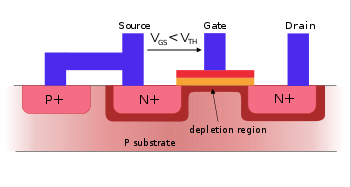
\includegraphics[width=0.6\textwidth,height=\textheight,keepaspectratio]{Krets_nMOS}
  \caption{Tverrsnitt av nMOS fra Wikipedia\label{fig:nMOS}}
\end{figure}

Til den éne gardinen kobles terminalen \textit{source} (S). Til den andre
gardinen \textit{drain} (D). Strøm klarer ikke å passere mellom dem til vanlig,
siden man får spenningsbarriærer mellom viduet og gardiene. En tredje terminal,
\textit{gate} (G) er koblet til en \textbf{metall}plate med et isolerende
\textbf{oksid}lag, som ``kobler'' source og drain. Gate er isolert, så det går
ikke faktisk strøm, men platen kan lades opp likt en kondensator, der vinduet er
den andre platen. Viduet må da være koblet opp til en fjerde terminal,
\textit{body} (B), slik at gate har en spenning å være relativ til. Når gate og
body har en spenningsforskjell riktig vei over terskelspenningen $V_{TH}$,
dannes en bru av positiv eller negativ ladning mellom gardinene. Avhengig av
dopingen lar én av disse strøm passere mellom source og drain.
%
Ofte har transistorer bare tre terminaler. Det er fordi body kobles opp til
source. Da måles gatespenning $V_{GS}$ relativt til sourcespenning $V_{S}$: \\
%
pMOS lukkes mellom \textit{source} og \textit{drain} når $V_{GS} \ll V_{S}$\\
nMOS lukkes mellom \textit{source} og \textit{drain} når $V_{GS} \gg V_{S}$\\
Her betyr $\ll$ en differanse på mer enn terskelspenningen $V_{TH}$. Eksempel på
terskelspenning: \SI{0.45}{\volt}.

\subsection{CMOS}\label{sec:cmos}
CMOS (Complementary Metal-oxide-semiconductor) er et system for design av
logiske kretser med MOSFET\@. Det baserer seg på symmetriske par av pMOS
og nMOS koblet opp til $V_{DD}$, $V_{SS}$, inputs og hverandre.
$V_{DD}$ er drain, og er høy (f.eks. \SI{5}{\volt}). $V_{SS}$ er source, som er
lav, altså jord.
%
\begin{figure}[hbt!]
    \centering
    \begin{circuitikz} \draw
    (0,1) node[pmos](ap){}
    (2,1) node[pmos](bp){}
    (1,-1) node[nmos](an){}
    (1,-2) node[nmos](bn){}

    (ap.S) -- ++(1,0) -- ++(0,.3) node[odiamondpole]{$V_{DD}$}
    (bp.S) -- ++(-1,0)

    (ap.G) node[left]{A}
    (bp.G) node[left]{B}
    (an.G) node[left]{A}
    (bn.G) node[left]{B}

    (bn.S) node[ground]{} node[below right]{$V_{SS}$}

    (ap.D) -- (0, 0) -- (4,0) node[odiamondpole]{Out}
    (bp.D) to[short,-*] (2,0)
    (an.D) to[short,-*] (1,0)
    ;
    \end{circuitikz}
    \caption{En NAND-port i CMOS \label{fig:CMOS_NAND}}
\end{figure}

%
CMOS følger regler for oppsett. En \textbf{pMOS} sin \textit{source} er alltid
koblet til $V_{DD}$ eller til en annen pMOS sin \textit{drain}. En \textbf{nMOS}
sin \textit{source} er alltid koblet til $V_{SS}$ eller til en annen nMOS sin
\textit{drain}\@. pMOS brukes altså til opptrekk av output, og nMOS brukes til
nedtrekk av output. \textit{Complementary} betyr at kun én av trekkene på output
kan være lukket. Se figur~\ref{fig:CMOS_NAND}.
%
\subsubsection{Viktig å huske om CMOS}
\begin{itemize}
  \item CMOS bruker kun strøm på å endre ladning i gate i MOSFETene. Det betyr at det
    kun går strøm til input når input endrer seg.
  \item $V_{DD}$ er drain, men er altså høy. $V_{SS}$ er source, men er altså
    lav/jord.
    \item En pMOS sin $source$-terminal kan aldri kobles til $V_{SS}$, men kan
    kobles til $V_{DD}$. En nMOS er omvendt. Dette gir mening med tanke på at
    $gate$ skal sammenlignes med $source$.
\end{itemize}

\newcommand{\varkern}{\hspace{0.06em}}
\newcommand{\var}[1]{\varkern#1\varkern}
\newcommand{\kom}[1]{\varkern\bar{#1}\varkern}
\newcommand{\xor}{\oplus}
\newcommand{\xnor}{\odot}

\section{Boolsk algebra}\label{sec:bool_alg}
I boolsk algebra er alle verdier enten 0 eller 1. Et boolsk uttrykk består av
slike boolske verdier og boolske operatorer. En boolsk funksjon tar parametere
og evaluerer til enten $0$ eller $1$. Funksjoner kan representeres både som et
boolsk uttrykk der parameterne forekommer som literaler ($x+yz$), og
som en sannhetstabell. Operatorer er i seg selv boolske funksjoner.

\subsection{Unary operatorer}
Unary betyr at operatoren er en funksjon med ett parameter.
Det finnes kun 4 unary operatorer $F(x)$ i boolsk algebra:
\begin{table}[H]
\centering
\begin{tabular}{ |c|C|C|C|c|c| }
  \toprule
  Navn & \text{Symbol} & \multicolumn{2}{|c|}{F for $\var{x}$=} & Uttrykk & Kommentar \\
  & & 0 & 1 & & \\
  \midrule
  Zero & & 0 & 0 & $F_{0} = \var{0}$ & Konstant 0 \\
  Ident. & \var{x} & 0 & 1 & $F_{1} = \var{x}$ & Identitet \\
  Compl. & \kom{x} \text{/} \var{x'} & 1 & 0 & $F_{2} = \kom{x}$ & Komplement \\
  One & & 1 & 1 & $F_{3} = \var{1}$ & Konstant 1 \\
  \bottomrule
\end{tabular}
\end{table}

\subsection{Binære operatorer}
Binære operatorer kalles binære fordi de tar inn to operander (ikke fordi
operandene er binære verdier). Det finnes $2^{2^{2}} = 16$ forskjellige boolske
funksjoner $F(x,y)$, men vi bryr oss ikke om alle.

\begin{table}[H]
\centering
\begin{tabular}{ |c|C|C|C|C|C|c|c| }
  \toprule
  Navn & \text{Symbol} & \multicolumn{4}{|c|}{F for $\var{x,y}$=} & Uttrykk & Kommentar \\
  & & 0,0 & 0,1 & 1,0 & 1,1 & & \\
  \midrule
  Zero & & 0 & 0 & 0 & 0 & $F_{0} = \var{0}$ & Konstant 0 \\
  AND & \var{x}\cdot\var{y} & 0 & 0 & 0 & 1 & $F_{1} = \var{x}\var{y}$ & x og y \\
  XOR & \var{x}\xor\var{y} & 0 & 1 & 1 & 0 & $F_{6} = \var{x}\kom{y}+\kom{x}\var{y}$ & enten x eller y \\
  OR & \var{x} + \var{y} & 0 & 1 & 1 & 1 & $F_{7} = \var{x}+\var{y}$ & x eller y \\
  NOR & \var{x}\downarrow\var{y} & 1 & 0 & 0 & 0 & $F_{8} = \overline{\var{x}+\var{y}}$ & Not-OR \\
  Equiv. & \var{x}\xnor\var{y} & 1 & 0 & 0 & 1 & $F_{9} = \var{x}\var{y}+\kom{x}\kom{y}$ & x = y \\
  NAND & \var{x}\uparrow\var{y} & 1 & 1 & 1 & 0 & $F_{14} = \overline{\var{x}\var{y}}$ & Not-AND \\
  One & & 1 & 1 & 1 & 1 & $F_{15} = 1$ & Konstant 1 \\
  \bottomrule
\end{tabular}
\end{table}

\subsection{Regneregler}
Vi har en rekke regneregler på operatorene i boolsk algebra. Med disse kan vi
omskrive boolske uttrykk til enklere eller tydeligere uttrykk. Alle boolske
uttrykk kan skrives som 

\subsubsection{De Morgans teoremer}
De Morgans teoremer gir oss en sammenheng mellom AND og OR, ved å invertere både
input og output.

\begin{center}
  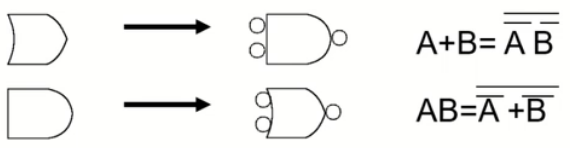
\includegraphics[width=0.6\textwidth,height=\textheight,keepaspectratio]{Krets_DeMorgan}
\end{center}

Hvis vi starter med komplementet gir dette oss følgende
\[\kom{x}\kom{y} = \overline{\var{x}+\var{y}}\]
\[\kom{x} + \kom{y} = \overline{\var{x}\var{y}}\]
Vi kan også gjøre flere i slengen:
\[\overline{\var{x} + \var{y} + \var{z}} = \kom{x}\kom{y}\kom{z}\]

\subsection{Forenkling av uttrykk}
Vi ser på representasjonformer og måter å forenkle boolske uttrykk i
seksjon~\ref{sec:bool_func} om boolske funksjoner.

\section{Logiske porter}\label{sec:logiske_porter}
Med CMOS (Seksjon~\ref{sec:cmos}) kan man lage porter som utfører logiske
operasjoner. Se tabell~\ref{tab:porter}. Portene bruker et visst antall
transistorer og har en forplantningsforsinkelse. Se
Seksjon~\ref{sec:tekonologimapping} om teknologimapping for effektiv bruk av
porter i logiske kretser.

\begin{figure}[hbt!]
  \centering
  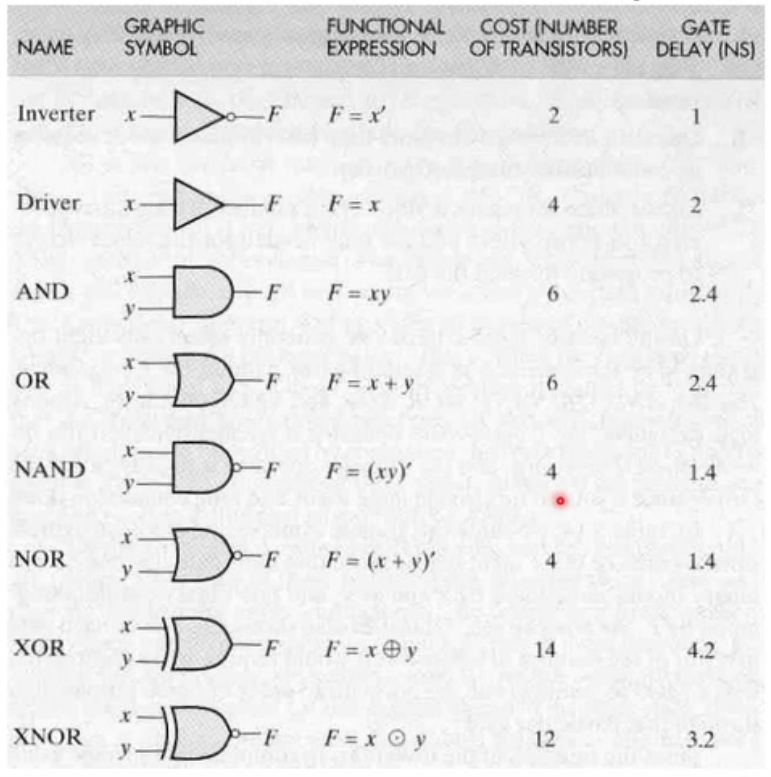
\includegraphics[width=\textwidth,height=\textheight,keepaspectratio]{Krets_Gates}
  \captionof{table}{Logiske porter, Figur 3.14 i Gajski\label{tab:porter}}
\end{figure}

\section{Forsinkelser}\label{sec:forsinkelser}
Komponenter har alltid en viss kapasitans som gjør at spenningsendriger ikke kan
skje momentant. Derfor må vi ta hensyn til forsinkelser, også i digitale
kretser, der signaler til tider vil befinne seg ``mellom'' $0$ og $1$. Vi
opererer med flere typer forsinkelser. For å finne verdiene for et gitt
komponent må vi se på komponentets datablad. Se seksjon~\ref{sec:datablader}.

\subsection{Eksempel med CMOS-inverter}
TODO\@: Sett inn eksempelet med CMOS-inverter og kondensatorer.

\subsection{Forplantningstid}
Forplantningstid (Propagation delay) er tiden det tar fra input har
endret seg, til output endrer seg. Oftest ser man på tiden det tar fra input har
passert $50\%$ til output passerer $50\%$. Man deler
forplantningstiden inn i $t_{PLH}$ (Output går lav til høy) og $t_{PHL}$ (Output
går høy til lav). Se figur~\ref{fig:delay}. Vi skiller mellom $t_{PHL}$ og
$t_{PLH}$ siden de kan være forskjellige, men vi har også
$t_{P} = \frac{t_{PHL}+t_{PLH}}{2}$ som vi bare kaller ``forsinkelse gjennom porten''.

\begin{figure}[hbt!]
  \centering
  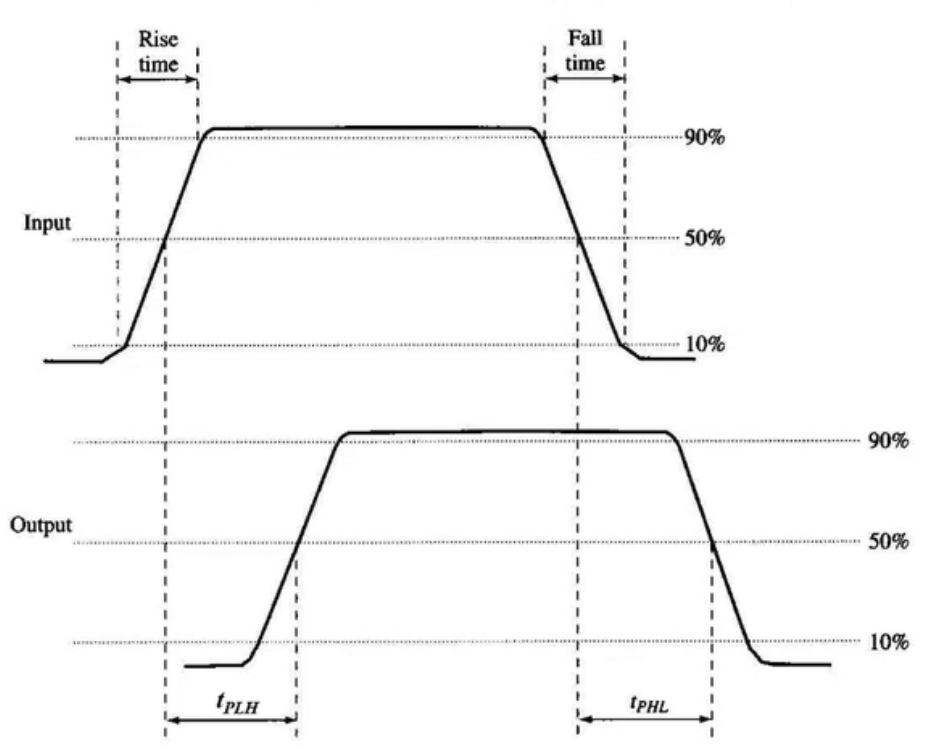
\includegraphics[width=0.8\textwidth,height=0.8\textheight,keepaspectratio]{Krets_Delay}
  \caption{Tider målt på en enkel port med input og output\label{fig:delay}}
\end{figure}

Forplantningstid måles gjerne i nanosekunder. En kobberledning har en typisk
forplantningstid rundt $\frac{1}{15}$\si[per-mode =
fraction]{\nano\second\per\centi\meter}. En enkeltsående IC-chip med XOR ved
$V_{DD}=\SI{5}{\volt}$ kan ha $t_{PLH} = \SI{140}{\nano\second}$. Merk
at porter i logiske kretser oppererer rundt 1--4\si{\nano\second}. Se
seksjon~\ref{sec:logiske_porter}.

\subsection{Stigetid}
Stigetid (Rise time) er hvor lang tid det tar fra signalet
er gått fra gyldig low-verdi til gyldig high-verdi. Verdien benevnes med
$t_{TLH}$. I forelesning har vi opperert med at $10\%$ er terskelen for lav, og
$90\%$ er terskelen for høy. Se figur~\ref{fig:delay}.

\subsection{Falltid}
Falltid (Fall time) er hvor land tid det motsatte tar, altså høy til lav.
Benevnes $t_{THL}$. Se figur~\ref{fig:delay}.

\subsection{Kritisk sti}\label{sec:kritisk_sti}
Når vi skal finne forplantningstid i en krets sammensatt av flere komponenter,
må vi først finne en kritisk sti, og to input-states som, når de veksles mellom,
forursaker at et signal må propageres gjennom hele den kritiske stien før output
endrer seg. Stien er valgt slik at tiden det tar før signalet når output er størst
mulig. For å finne forplantningstiden til den kritiske stien kan vi måle input og
output, og ta tiden fra input endres til output endres. Husk at
forplantningsstid måles fra signalet passerer $50\%$ på input til det passerer
$50\%$ av sluttoutput. Ofte vil å endre kun én input-bit gi kritisk sti, så
fremt de andre er satt riktig.

For logiske kretser med porter har vi fått oppgitt en tabell med \textit{gate
 delay} for hver port. Se seksjon~\ref{sec:logiske_porter}. Da slipper vi å
forholde oss til $t_{PLH}$ og $t_{PHL}$, og kan bare addere sammen
forsinkelsene til hvert komponent på den tregeste veien fra en input til en
output. Se figur~\ref{fig:kritisk_sti}. Gjennom boolsk algebra er det kanskje
mulig å forbedre tiden til kritisk sti. Se seksjon~\ref{sec:tekonologimapping}
om Teknologimapping.

\begin{figure}[hbt!]
  \centering
  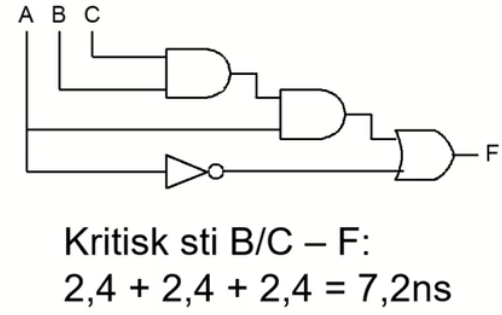
\includegraphics[width=0.6\textwidth,height=\textheight,keepaspectratio]{Krets_DuringTeknomap}
  \caption{Regning på kritisk sti i enkel logisk krets\label{fig:kritisk_sti}}
\end{figure}

Husk at datablader for chipper gjerne opererer både med $Typ$, $Min$ og
$Max$-verdier for forplantningstid. Variasjon i tid kan skyldes flere ting, slik
som temperatur og kapasitans i komponenter koblet til output. Når vi ser på
portkretser i dette faget har vi forenklet regningen, og forholder oss kun til
ett tall for forplantningstid.

\section{Binærtall}
TODO\@: Bruke 2-tallssystemet.

\subsection{Konvertere fra binærtall}
TODO

\subsection{Konvertere til binærtall}
TODO

\subsection{Desimaltall og andre tallsystemer}
TODO

\subsection{Graykoding}
Graykoding, også kjent som ``reflected binary'', er en binær koding av tall der alle
nabotall har nøyaktig én bit forskjell. Man kan omdanne binærtall til og fra
Graykoding. Huskeregel: $G = B \xor (B >> 1)$.
\begin{figure}[H]
  \centering
  \begin{subfigure}{.4\textwidth}
    \centering
    \begin{align*}
      G_{7} &= B_{7} \\
      G_{6} &= B_{7} \xor B_{6} \\
            &\vdots \\
      G_{0} &= B_{1} \xor B_{0} \\
    \end{align*}
    \caption{Graykoding fra binær}
  \end{subfigure}
  \begin{subfigure}{.4\textwidth}
    \centering
    \begin{align*}
      B_{7} &= G_{7} \\
      B_{6} &= B_{7} \xor G_{6} \\
            &\vdots \\
      B_{0} &= B_{1} \xor G_{0} \\
    \end{align*}
    \caption{Binær fra graykoding}
  \end{subfigure}
  \caption{Omgjøring av 8-bit til og fra graykoding}
\end{figure}

\section{Negative binærtall}
Med binærtall kan vi representere tall som strenger av $0$ og $1$, som er veldig
praktisk i digitale kretser. I denne seksjonen skal vi vise hvordan også
negative tall kan representeres.

\subsection{Signed magnitude}
Dersom vi i det daglige vil representere negative tall, pleier vi å legge på et
\textbf{--}~-tegn foran tallet. For at dette skal passe i en digital krets, kan vi
si at MSB bestemmer fortegnet til tallet, og resten av bit-ene fungerer som
normalt. Dette kalles signed magnitude. Konvensjonen er at $1$ er \textbf{-} og
$0$ er \textbf{+}.
\begin{center}
  Eksempler på 8-bits signed magnitude\\[5mm]
  \begin{tabular}{c|c}
    \toprule
    Signed magnitude & Tallverdi \\
    \midrule
    00000101 & 5 \\
    10000101 & -5 \\
    01111111 & 127 \\
    11111111 & -127 \\
    00000000 & 0 \\
    10000000 & -0 \\
    \bottomrule
  \end{tabular}
\end{center}

8-bits signed magnitude kan altså representere tall i intervallet $\lbrack-127, 127\rbrack$.
Merk at $+0$ og $-0$ har ulike representasjoner, selv om de egentlig er samme tall.

\subsection{Toerkomplement}
Toerkomplement er veldig likt som vanlig binærtall, bortsett fra at mest
signifikante bit (MSB) ikke representerer $2^{n-1}$, men $-2^{n-1}$, der $n$ er
antall bits i representasjonen. Dersom MSB er $0$ vil det representerte tallet være
akkurat det samme som i vanlig binærtall. Hvis MSB er $1$ er tallet negativt.
Eksempel:
%
\begin{align*}
  10010110 &= 1 \cdot -2^7 + 0 \cdot 2^6 + 0 \cdot 2^5 + 1 \cdot 2^4 + 0 \cdot 2^3 + 1 \cdot 2^2 + 1 \cdot 2^1 + 0 \cdot 2^0 \\
             &= -128 + 16 + 4 + 2 \\
             &= -106
\end{align*}
%
Fordelen med toerkomplementsrepresentasjon er at mange operasjoner støtter
representasjonen uten vidre. Vi vet fra før at en f.eks. 16-bits-representasjon
er en ekvivalensklasse modulo $2^{16}$, siden all eventuell overflow forsvinner
fra representasjonen. Observer at
\[2^{15} \equiv -2^{15} \mod 2^{16}\]
Endringen vi har gjort til betydningen av MSB har altså ingenting å si modulo
$2^{16}$. Det betyr at addisjon mellom $5$ og $-2$ gir oss $3$, uten at
addisjonskretsen trenger å vite om toerkomplement. Toerkomplementet er det man
automatisk får hvis man subtraherer et tall fra $0$ og ignorerer overflow.

\begin{center}
  Eksempler på 8-bits toerkomplementsrepresentasjon\\[5mm]
  \begin{tabular}{c|c}
    \toprule
    Toerkomplement & Tallverdi \\
    \midrule
    00000010 & 2 \\
    11111110 & -2 \\
    11111111 & -1 \\
    00010100 & 20 \\
    11101100 & -20 \\
    00010101 & 21 \\
    11101011 & -21 \\
    01111111 & 127 \\
    10000001 & -127 \\
    10000000 & -128 \\
    \bottomrule
  \end{tabular}
\end{center}

8-bits toerkomplement kan altså representere tall i invervallet $\lbrack-128,127\rbrack$,
som er én mer enn signed magnitude. Dette er fordi vi ikke lenger har ulike
representasjoner for $-0$ og $+0$.

\subsubsection{Toerkomplement-operasjonen}\label{sec:toerkomplement-op}
Egentlig er toerkomplement navnet på en operasjon. Operasjonen er definert slik
at et binærtall på $n$ bits og dets toerkomplement blir $2^n$ i sum. Merk at
$2^n \equiv 0 \mod 2^n$, så vi kan også si at et tall og dets toerkomplement blir $0$
i sum når overflow forkastes.

Denne operasjonen vil derfor i praksis være å omgjøre et tall på
toerkomplementsform til motsatt fortegn. $4$ blir $-4$ og omvendt. Denne
operasjonen er ikke bare å flippe MSB, slik som i signed magnitude. Alle bits må
flippes, og deretter må $1$ legges til. Overflow ignoreres.

\textbf{Merk.} $10000000$ ($-128$) blir til seg selv når man
tar 8-bits toerkomplement. Dette er fordi $+128$ ikke kan representeres i 8-bits
toerkomplementform.

En mer mennesketilpasset måte: Begynn med minst signifikante bit (LSB) og beveg
deg oppover til du møter en bit som er $1$. Alle påfølgende bits (opp til og med
MSB) flippes. Eksempel: Hva er $11010100$ i 10-tallsystemet?
%
\begin{align*}
  &11010100 \\
  \Rightarrow - &00101100_2 & \text{Toerkomplementet} \\
  \Rightarrow - &(32_{10} + 8_{10} + 4_{10}) \\
  \Rightarrow - &44_{10}
\end{align*}

\subsubsection{Endring av antall bits}
Gitt et tall på $n$-bits toerkomplementsform, vil vi ofte kunne ønske samme tall
representert med en annen mengde bits. For å øke antall bits med $k$ kopierer vi
MSB $k$ ganger og legger dem på venstresiden.
\begin{align*}
  1101 &\Rightarrow 11111101 \\
  0110 &\Rightarrow 00000110
\end{align*}

For å senke antall bits fjerner vi \textit{MSB}. Vi kan kun fjerne \textit{MSB}
så lenge den nye \textit{MSB} er det samme som den vi fjernet. Hvis vi fjerner
flere bits enn det har vi ikke nok bits til å representere tallet.
\begin{align*}
  11110101 &\Rightarrow 10101 \\
  00001101 &\Rightarrow 01101
\end{align*}

\section{Regning med binærtall}
Binærtall er kun en representasjonsform av tall, så $6+7$ er $13$ uansett
hvilket tallsystem man bruker. Likevel er det kjekt å kunne regne med tallene
direkte i binærtall på toerkomplementsform, siden det er slik de gjerne
representeres i kretser. I tillegg har vi en endelig mengde bits, så det er ikke
alle tall som kan representeres. Hvis vi har for få bits blir kanskje $6+7 = -3$.

\subsection{Absoluttverdi}
Dersom \textit{MSB} er 1, gjør toerkomplementoperasjonen. Se Seksjon~\ref{sec:toerkomplement-op}.

\subsection{Addisjon}
Addisjon fungerer veldig likt som man ville gjort på papir i 10-tallssystemet.
Vi skriver tallene under hverandre, og adderer bortover fra LSB til MSB. Hvis
begge tallene er $1$ får vi $1$ i mente, og må ta den med vidre. Eksempel med
8-bits tall:

\begin{center}
  \begin{tabular}{rlr}
     &11010100 & -44 \\
    +&01110110 & 118 \\
    \midrule
    =&01001010 & 74
  \end{tabular}
\end{center}

I dette tilfellet ble carry ut av MSB $1$. Dette betyr ikke at vi overflowet.
Addisjonen har overflowet hvis to positive tall ble negative i sum, eller to
negative ble positive i sum. Summen av et positivt og negativt tall kan aldri
overflowe.  

\subsection{Subtraksjon}
Subtraksjon gjøres gjerne ved å ta toerkomplementet til tallet som skal
subtraheres, og gjøre addisjon.

\subsection{Multiplikasjon}
Multiplikasjon kan gjøres ved å først ta absoluttverdien av faktorene,
multiplisere, og til slutt sette riktig fortegn på resultatet. I dette faget
lærer vi en metode som fungerer generelt både på positive og negative tall på
toerkomplementsform. Vi bruker $-14 \times (-5)$ som eksempel, og bruker $5$-bits
input.
\newcommand{\mult}{\red{1}\green{1}\maroon{0}\orange{1}\purple{1}}
%
\[10010 \times \mult\]
%
Vi kaller den første faktoren multiplikand, og den andre multiplikator. Når vi
multipliserer et $m$-bits tall med et $n$-bits tall blir produktet et $m+n$-bits
tall. Det første vi gjør er å utvide multiplikanden til like mange bits som
resultatet, ved å kopiere MSB $n$ ganger.
%
\[1111110010 \times \mult\]
%
Multiplikasjon er gjentatt addisjon. For å holde orden på resultatet underveis
bruker vi en variabel vi kaller \textit{partielt produkt}. Til å begynne med er
den $m+n$ bits med $0$.
\[0000000000\]
Deretter går vi gjennom hver bit i multiplikatoren, og for hver $1$-bit adderer
vi multiplikanden til partielt produkt. Vi skifter multiplikanden til venstre
for hver bit vi går opp i multiplikatoren. Dette er fordi bit $k$ i
multiplikatoren representerer $2^k$. MSB i multiplikatoren er spesiell i
toerkomplementsrepresentasjon, så den representerer $-2^4$. Dette gjør vi i
praksis ved å ta toerkomplementet til multiplikanden i siste rad.

\begin{center}
  \begin{tabular}{ll}
    $\blue{1111110010} \times \mult$ & $(-14)\times(-5)$ \\
    \midrule
    0000000000 & partielt produkt \\
    \blue{1111110010} & multiplikand $\times\ 2^0 \times \purple{1}$ \\
    \midrule
    1111110010 & partielt produkt \\
    \blue{111110010}0 & multiplikand $\times\ 2^1 \times \orange{1}$ \\
    \midrule
    1111010110 & partielt produkt \\
    \blue{00000000}00 & multiplikand $\times\ 2^2 \times \maroon{0}$ \\
    \midrule
    1111010110 & partielt produkt \\
    \blue{1110010}000 & multiplikand $\times\ 2^3 \times \green{1}$ \\
    \midrule
    1101100110 & partielt produkt \\
    \blue{001110}0000 & multiplikand $\times\ {-2^4} \times \red{1}$ \\
    \midrule
    0001000110 & $70_{10}$ \\
    \bottomrule
    \bottomrule
  \end{tabular}
\end{center}

Vi ignorerer all overflow på partielt produkt underveis, siden vi vet at svaret
blir et $10$-bits tall.

\subsection{Divisjon}
Gjøres som vanlig, bruk fantasien TODO.

\section{Boolske funksjoner}\label{sec:bool_func}
Denne seksjonen inneholder måter å representere boolske funksjoner på, og
algebra for å forenkle boolske uttrykk med flere variabler. Husk De Morgans
teoremer og slikt fra seksjon~\ref{sec:bool_alg}.

\subsection{Kanoniske former}
Et boolsk uttrykk på kanonisk form består enten av OR av ANDer, eller som AND av ORer.
Alle variabler må forekomme i hvert ``ledd'', enten som ikke-komplementær eller
komplementær. Vi kan bruke boolsk algebra for å omdanne et vilkårlig uttrykk til
kanonisk form:
\[\kom{x}\kom{y} + \var{x}\var{y}\var{z} = \kom{x}\kom{y}(\var{z} + \kom{z}) +
  \var{x}\var{y}\var{z} =  \kom{x}\kom{y}\var{z} + \kom{x}\kom{y}\kom{z} + \var{x}\var{y}\var{z}\]
Vi har da gjort uttrykket om til OR av ledd der hvert ledd er ANDet og
inneholder alle variabler. Vi kaller dette oppsettet SOP, \textit{Sum of
  Products}. For en gitt boolsk funksjon finnes det nøyaktig én kanonisk SOP og
én kanonisk POS, \textit{Product of sum}. Disse leddene kalles henholdsvis
mintermer og makstermer.

\subsubsection{Minterm}
AND av alle variabler på enten komplementær eller ikke-komplementær form.
Indeksen til mintermen forteller hvilke variabler som er på ikke-komplementær
form. MSB av indeks svarer til første variabel, og LSB til siste. Hvis bit-en er
$0$ blir variablen på komplementær form. Se tabell~\ref{table:minterm}.

\begin{table}[H]
  \centering
  \begin{tabular}{| C | C | C |}
    \toprule
\text{Minterm} & \text{Indeks} & \text{Uttrykk} \\
    \midrule
    m_{0} & 000_{(2)} & \kom{x} \kom{y} \kom{z} \\
    m_{1} & 001_{(2)} & \kom{x} \kom{y} \var{z} \\
    m_{2} & 010_{(2)} & \kom{x} \var{y} \kom{z} \\
    \vdots & \vdots & \vdots \\
    m_{7} & 111_{(2)} & \var{x} \var{y} \var{z} \\
    \bottomrule
  \end{tabular}
  \caption{Eksempel med tre variabler $x$, $y$ og $z$\label{table:minterm}}
\end{table}

\noindent
Vi kan da omdanne en sannehetstabell til kanonisk form ved å se på hvilke rader
som gir 1, og ORe sammen mintermene til de radene. Hvis ingen av mintermene er
perfekt tilfredsstilt, blir ingen ledd 1, og uttrykket blir 0. Mintermen $m_{6}$
er altså tilfredsstilt hvis og bare hvis $(x,y,z)=(1,1,0)$.

\begin{table}[H]
  \centering
  \begin{tabular}{|c|C|C|C|C|}
    \toprule
    indeks & x & y & z & F(x,y,z) \\
    \midrule
    0 & 0 & 0 & 0 & 1 \\
    1 & 0 & 0 & 1 & 1 \\
    2 & 0 & 1 & 0 & 0 \\
    3 & 0 & 1 & 1 & 0 \\
    4 & 1 & 0 & 0 & 0 \\
    5 & 1 & 0 & 1 & 1 \\
    6 & 1 & 1 & 0 & 0 \\
    7 & 1 & 1 & 1 & 1 \\
    \bottomrule
  \end{tabular}
  \caption{Sannhetstabell for F(x,y,z)}
\end{table}

\noindent
Vi kan nå skrive F som summen av mintermene som representerer radene der $F=1$
\[F = \kom{x}\kom{y}\kom{z} + \kom{x}\kom{y}\var{z} + \var{x}\kom{y}\var{z} + \var{x}\var{y}\var{z} = m_{0}+m_{1}+m_{5}+m_{7} = \Sigma(0,1,5,7)\]
$\Sigma$ betyr altså OR av mintermene med gitt indeks.

\subsubsection{Maxterm}
OR av alle variabler på enten ikke-komplementær eller komplementær form.
\begin{center}
\begin{tabular}{ C C C }
  M_{0} & 000_{(2)} & \var{x} + \var{y} + \var{z} \\
  M_{1} & 001_{(2)} & \var{x} + \var{y} + \kom{z} \\
  M_{2} & 010_{(2)} & \var{x} + \kom{y} + \var{z} \\
  \vdots & \vdots & \vdots \\
  M_{7} & 111_{(2)} & \kom{x} + \kom{y} + \kom{z}
\end{tabular}
\end{center}
Vi kan da omdanne en sannehetstabell til kanonisk form ved å se på hvilke rader
som gir 0, og ANDe sammen maxtermene for de radene. For at en maxterm skal være
0 må den passe med raden på en prikk. Hvis noen av radene passer,
blir produktet av makstermene 0, ellers 1.

\[F = (\var{x}+\kom{y}+\var{z})(\kom{x}+\var{y}+\kom{z})(\kom{x}+\kom{y}+\var{z}) = \Pi(2,5,6)\]
$\Pi$ betyr altså AND av maxtermene med gitt indeks.

\subsubsection{Regler}
Mintermen $m_{3} = \kom{x}\var{y}\var{z}$ er kun $1$ når $(x,y,z) = (0,1,1)$ \\
Maxtermen $M_{3} = \var{x}+\kom{y}+\kom{z}$ er kun $0$ når $(x,y,z) = (0,1,1)$
%
Min tar laveste tall, er detfor AND\@. Minterm er derfor kun $1$ under riktig
omstendighet. Max tar høyeste tall, er derfor OR\@. Maxterm derfor kun $0$ under
riktig omstendighet.

\textbf{Algebra med $\Sigma$ og $\Pi$}\\
For en funksjon $F(x,y,z)$ (8 forskjellige mintermer og maxtermer)
\begin{align*}
  \Sigma(1,3,5) &= \overline{\Sigma(0,2,4,6,7)} \\
           &= \Pi(0,2,4,6,7) \\
           &= \overline{\Pi(1,3,5)}
\end{align*}

For eksempel på bruk av minterm, se seksjon~\ref{sec:fulladder} om å lage
funskoner og krets for fulladderer.

\subsection{Standardform}
Standardform er ikke like streng som kanonisk form, og vi trenger ikke nevne alle
variabler i hvert ledd. Vi må likevel forholde oss til sum av produkt (SOP)
eller produkt av sum (POS).

\[F = \var{x}\var{y} + \var{x}\kom{y}\var{z} + \kom{x}\var{y}\var{z}\]

Hvert produkt her kalles en implikant.

\subsubsection{Literalreduksjon}
Vi kan redusere antall literaler ved å gjøre algebra.
\begin{align*}
  F &= \var{x}\var{y} + \var{x}\kom{y}\var{z} + \kom{x}\var{y}\var{z} \\
    &= \var{x}\var{y}\var{z} + \var{x}\var{y}\kom{z} + \var{x}\kom{y}\var{z} + \kom{x}\var{y}\var{z} \\
    &= \var{x}\var{y}\var{z} + \var{x}\var{y}\kom{z} + \var{x}\var{y}\var{z} + \var{x}\kom{y}\var{z} + \var{x}\var{y}\var{z} + \kom{x}\var{y}\var{z} \\
    &= \var{x}\var{y}(\var{z} + \kom{z}) + \var{x}(\var{y} + \kom{y})\var{z} + (\var{x} + \kom{x})\var{y}\var{z} \\
    &= \var{x}\var{y} + \var{x}\var{z} + \var{y}\var{z}
\end{align*}
Vi har nå redusert antall literaler ned til en enklere SOP, men den kan
reduseres ytterligere.
\[\var{x}\var{y} + \var{x}\var{z} + \var{y}\var{z} = \var{x}(\var{y} + \var{z}) + \var{y}\var{z}\]
Dette er derimot ikke lenger en SOP, men en Sum av Produkt av Sum. Det er derfor
ingen grunn til å tro at kretsen blir noe raskere (snarere tvert imot), selv om
man har redusert antall literaler.

\subsubsection{Bytte mellom POS og SOP}
Akkurat som med mintermer og maxtermer kan vi bytte mellom SOP og POS ved å ta
inversen til uttrykket og bruke DeMorgans.

\begin{align*}
  F &= \var{x}\var{y} + \var{x}\kom{y}\var{z} + \kom{x}\var{y}\var{z} \\
  \bar{F} &= \overline{\var{x}\var{y} + \var{x}\kom{y}\var{z} + \kom{x}\var{y}\var{z}} \\
    &= (\overline{\var{x}\var{y}})(\overline{\var{x}\kom{y}\var{z}})(\overline{\kom{x}\var{y}\var{z}}) \\
    &= (\kom{x} + \kom{y})(\kom{x}+\var{y}+\kom{z})(\var{x}+\kom{y}+\kom{z})
\end{align*}

Dette bruker vi i PAL. Se Seksjon~\ref{sec:PAL}.

\subsection{Karnaughdiagram}
TODO\@:Skriv

\subsection{Tabellmetoden (Quine-McCluskey)}
TODO\@:Skriv. Her er engelsk Wikipedia egentlig veldig god.

\subsubsection{Elementære primledd}
Dette er ledd som garantert burde være med i SOP av utrykket.

\section{Datablader}\label{sec:datablader}
Datablader forteller oss egenskapene til komponenter når de skal brukes i kretser.
Tallene i databladene forutsetter visse omstendigheter, gjerne definert i toppen
av tabellen. Dette kan være temperatur $T_{A}$, lastkapasitans $C_{L}$ og gitt
resistiv last $R_{L}$. Databladene forutsetter også at innsignaler innfrir noen
oppgitte krav til stigetid og falltid ($t_{TLH}$, $t_{THL}$), og at spenninger
er innenfor tilatte skranker.

\subsection{Oppgitte verdier}
\textbf{Forplantingstid}, \textbf{Stigetid}, og \textbf{Falltid}\\
Disse forsinkelsene kalles henholdsvis $t_{PLH}$/$t_{PHL}$, $t_{TLH}$ og
$t_{THL}$. Se seksjon~\ref{sec:forsinkelser} om forsinkelser.

\textbf{Inputkapasitans}\\
Input har en viss kapasitans $C_{in}$, altså må en viss mengde strøm tilføres for å endre
spenningen opp til høy, eller motsatt for høy til lav.

\textbf{Gyldige spenninger}\\
$V_{DD}$ er driftspenningen, og andre egenskaper påvirkes av driftsspenningen.
$V_{IL}$ er hvilken skranke en input-spenning må ligge i for å anerkjennes som
lav. $V_{IH}$ er skranken for høy input-spenning.

\section{Logiske kretser}\label{sec:logic_circuits}
Nå skal vi bruke det vi vet om sannhetstabeller, algebra, porter og forsinkelse
til å lage kretser som utfører boolske funskjoner raskt og med få transistorer.

\subsection{1-bit fulladder}
TODO:\ Skriv.

\subsection{Ripple-carry fulladder}\label{sec:ripple_carry_fulladder}
Én måte å addere sammen to $n$-bits tall er å bruke $n$ 1-bits full-addere, med
carry propagert fra LSB oppover til MSB\@. Svaret blir et $n$-bits tall med
carry. Dette ligner måten addisjon gjøres for hånd. Problemet med denne adderen
er at carry må propageres helt fra LSB til MSB, og kritisk sti blir veldig lang.
(Hint: $0b11111111 + 1$)

\subsection{Carry-lookahead adder}
TODO:\ Skriv

\subsection{Adder-subtractor}\label{sec:adder-subtractor}
For å regne $x-y$ gjør vi istedet $x+(-y)$. Vi tar altså toskomplementet til $y$
og gjør en vanlig addisjon. Vi kan lett lage en krets som støtter både addisjon
og subtraksjon, ved å utvide en adder med en ekstra kontrollinput $SUB$. Dette
kalles en \textit{Adder-subtractor}

Å ta toskomplementet er i praksis åinvertere alle bits i $y$ og legge til $1$.
For å selektivt invertere XORer vi $SUB$ med alle bits i $y$. For å legge til $1$
trenger vi ikke en ekstra adder, men kan bruke carry-in i addisjonskretsen vi
allerede har. Se Figur~\ref{fig:adder-subtractor}.

\begin{figure}[hbt!]
  \centering
  \begin{circuitikz} \draw
    
    ;
  \end{circuitikz}
  \caption{16-bits Adder-subtractor\label{fig:adder-subtractor}}
\end{figure}

\subsection{Multiplekser}
En multiplekser er et kombinatorisk komponent som kan velge mellom flere inputsignaler å sende
vidre som outputsignal. En kontrollinput brukes for å velge mellom inputene. 
Dataen kan være enkeltsignaler eller fler-bits data. For blokkdiagramform og sannhetstabell, se
Figur~\ref{fig:multiplekser-blokk} og Tabell~\ref{tab:multiplekser-sannhet}.
\begin{figure}[hbt!]
  \centering
  \begin{minipage}{0.6\textwidth}
    \centering
    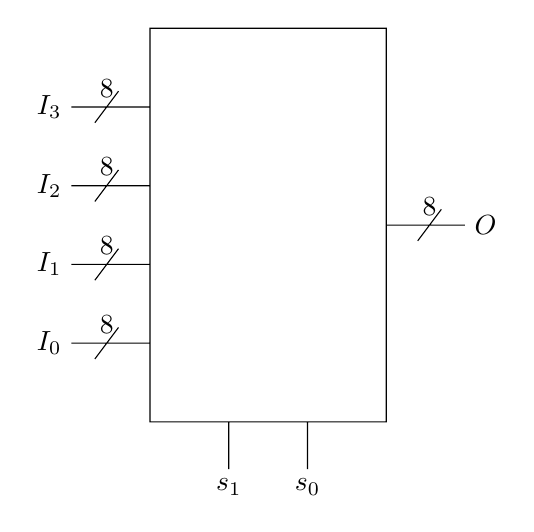
\begin{tikzpicture} \draw
      (0,0) rectangle (3,5)
      (0,1) -- ++(-1,0) node[left]{$I_0$} ++(.3,-.2) -- ++(.3,.4) node[midway, above]{8}
      (0,2) -- ++(-1,0) node[left]{$I_1$} ++(.3,-.2) -- ++(.3,.4) node[midway, above]{8}
      (0,3) -- ++(-1,0) node[left]{$I_2$} ++(.3,-.2) -- ++(.3,.4) node[midway, above]{8}
      (0,4) -- ++(-1,0) node[left]{$I_3$} ++(.3,-.2) -- ++(.3,.4) node[midway, above]{8}
      (1,0) - ++(0,-.6) node[below]{$s_1$}
      (2,0) - ++(0,-.6) node[below]{$s_0$}
      (3,2.5) -- ++(1,0) node[right]{$O$} ++(-.3,.2) -- ++(-.3,-.4) node[midway, above]{8}
      ;
    \end{tikzpicture}
    \caption{8-bits 4-kanal multiplekser\label{fig:multiplekser-blokk}}
  \end{minipage}
  \begin{minipage}{0.3\textwidth}
    \centering
    \begin{tabular}{cc|c}
      \toprule
      $s_1$ & $s_0$ & $O$ \\
      \midrule
      0 & 0 & $I_0$ \\
      0 & 1 & $I_1$ \\
      1 & 0 & $I_2$ \\
      1 & 1 & $I_3$ \\
      \bottomrule
    \end{tabular}
    \captionof{table}{Output fra 4-kanals multiplekser\label{tab:multiplekser-sannhet}}
  \end{minipage}
\end{figure}

Vi kaller en 4-kanals multiplekser for en 4x1. Dersom vi vil lage en
8x1 kan vi koble output fra to 4x1-multipleksere sammen som hver sin
input til en 2x1-multiplekser, og fordele $s_0$, $s_1$ og $s_2$. Slik
kan vi velge mellom alle 8 inputs.

\subsubsection{Logisk krets for 1-bits 2x1}\label{sec:logisk-krets-2x1}
For å gjøre det enkelt viser vi kun portdiagrammet for en enkel
2x1-multiplekser med enkle 1-bits inputs. Se Figur~\ref{fig:2x1}.

\begin{figure}[hbt!]
  \centering
  \begin{circuitikz} \draw
    (0,0) node[left]{$s_0$} to[short,-*] ++(1,0) coordinate(s)
    (4,1) node[american and port](and0){}
    (4,-1) node[american and port](and1){}
    (and0.in 2) ++(-.8,-.3) node[american not port](inv){}
    (and0.in 2)--(and0.in 2 -| inv.out) -- (inv.out)
    (inv.in)--(inv.in -| s) -- (s)
    (and1.in 1) -- (and1.in 1 -| s) --(s)
    (and0.in 1) -- (and0.in 1 -| 0,0) node[left]{$I_0$}
    (and1.in 2) -- (and1.in 2 -| 0,0) node[left]{$I_1$}
    (6,0) node[american or port](or){}
    (and0.out) -- (and0.out -| or.in 1) -- (or.in 1)
    (and1.out) -- (and1.out -| or.in 2) -- (or.in 2)
    (or.out) -- ++(1,0) node[right]{$O$}
    ;
  \end{circuitikz}
  \caption{Portdiagram for 2x1-multiplekser\label{fig:2x1}}
\end{figure}

Vi bruker denne kretsen som eksempel på teknologimapping i Seksjon~\ref{sec:tekonologimapping}.

\section{Teknologimapping}\label{sec:tekonologimapping}
NAND er en universell port, som betyr at alle boolske funksjoner kan
implementeres som kun NAND. Det samme gjelder NOR. I tillegg har NAND og NOR en
forplantningstid på \SI{1,4}{\nano\second}, og bruker kun $4$ transistorer hver.
Teknologimapping handler om å modifisere en logisk krets slik at den kun bruker
et sett tilgjengelige porter, og samtidig prøve å minimere kritisk sti og antall
transistorer. Dette gjøres gjennom å dekomponere porter med flere innganger, og
konvertering mellom porter med boolsk algebra. Siden AND er assosiativ kan en
3-inputs AND $xyz$ omdannes til to 2-inputs AND $(xy)z$. Vidre kan vi bruke
boolsk algebra for å omdanne porter.

\begin{align*}
  \var{x}\var{y} &= \overline{\overline{\var{x}\var{y}}} & \text{AND = NOT
                                                           NAND} \\
  \var{x}+\var{y} &= \overline{\overline{\var{x}+\var{y}}} & \text{OR = NOT
                                                           NOR} \\
  \var{x}+\var{y} &= \overline{\kom{x}\kom{y}} & \text{OR = NAND av NOT} \\
  \var{x}\var{y} &= \overline{\kom{x}+\kom{y}} & \text{AND = NOR av NOT} \\
  \overline{\kom{x}} &= \var{x} & \text{NOT NOT kanselleres}
\end{align*}

\subsection{2x1 med kun NAND og NOT}

Vi henter frem den logiske kretsen for en 2x1-multiplekser fra
Seksjon~\ref{sec:logisk-krets-2x1}. Ingen porter har mer enn 2 inputs, så vi
trenger ikke dekomponere.

\begin{center}
  \begin{circuitikz} \draw
    (0,0) node[left]{$s_0$} to[short,-*] ++(1,0) coordinate(s)
    (4,1) node[american and port](and0){}
    (4,-1) node[american and port](and1){}
    (and0.in 2) ++(-.8,-.3) node[american not port](inv){}
    (and0.in 2)--(and0.in 2 -| inv.out) -- (inv.out)
    (inv.in)--(inv.in -| s) -- (s)
    (and1.in 1) -- (and1.in 1 -| s) --(s)
    (and0.in 1) -- (and0.in 1 -| 0,0) node[left]{$I_0$}
    (and1.in 2) -- (and1.in 2 -| 0,0) node[left]{$I_1$}
    (6,0) node[american or port](or){}
    (and0.out) -- (and0.out -| or.in 1) -- (or.in 1)
    (and1.out) -- (and1.out -| or.in 2) -- (or.in 2)
    (or.out) -- ++(1,0) node[right]{$O$}
    ;
  \end{circuitikz}
\end{center}

Vi bruker tabell~\ref{tab:porter} for å regne ut antall transistorer og
propageringsforsinkelse gjennom kritisk sti. Før teknologimapping bruker vi $2+6+6+6=20$
transistorer og har en kritisk sti på $1+2,4+2,4 = \SI{5,8}{\nano\second}$.

Vi starter med å omdanne AND til NOT NAND, og bruker DeMorgan på OR-porten.
\[x + y = \overline{\kom{x}\kom{y}}\]
Dette gir oss følgende krets:

\begin{center}
  \begin{circuitikz} \draw
    (0,0) node[left]{$s_0$} to[short,-*] ++(1,0) coordinate(s)
    (4,1) node[american nand port](and0){}
    (4,-1) node[american nand port](and1){}
    (and0.in 2) ++(-.8,-.3) node[american not port](inv){}
    (and0.in 2)--(and0.in 2 -| inv.out) -- (inv.out)
    (inv.in)--(inv.in -| s) -- (s)
    (and1.in 1) -- (and1.in 1 -| s) --(s)
    (and0.in 1) -- (and0.in 1 -| 0,0) node[left]{$I_0$}
    (and1.in 2) -- (and1.in 2 -| 0,0) node[left]{$I_1$}

    (and0.out) ++ (1,0) node[american not port](not00){} ++ (1.4,0) node[american not port](not01){}
    (and1.out) ++ (1,0) node[american not port](not10){} ++ (1.4,0) node[american not port](not11){}

    (and0.out) -- (not00.in)
    (and1.out) -- (not10.in)
    
    (not00.out) -- (not01.in)
    (not10.out) -- (not11.in)
    
    (9,0) node[american nand port](or){}
    
    (not01.out) -- (and0.out -| or.in 1) -- (or.in 1)
    (not11.out) -- (and1.out -| or.in 2) -- (or.in 2)
    (or.out) -- ++(1,0) node[right]{$O$}
    ;
  \end{circuitikz}
\end{center}

Deretter fjerner vi doble invertere, siden $\overline{\kom{x}} = x$.

\begin{center}
  \begin{circuitikz} \draw
    (0,0) node[left]{$s_0$} to[short,-*] ++(1,0) coordinate(s)
    (4,1) node[american nand port](and0){}
    (4,-1) node[american nand port](and1){}
    (and0.in 2) ++(-.8,-.3) node[american not port](inv){}
    (and0.in 2)--(and0.in 2 -| inv.out) -- (inv.out)
    (inv.in)--(inv.in -| s) -- (s)
    (and1.in 1) -- (and1.in 1 -| s) --(s)
    (and0.in 1) -- (and0.in 1 -| 0,0) node[left]{$I_0$}
    (and1.in 2) -- (and1.in 2 -| 0,0) node[left]{$I_1$}
    (6,0) node[american nand port](or){}
    (and0.out) -- (and0.out -| or.in 1) -- (or.in 1)
    (and1.out) -- (and1.out -| or.in 2) -- (or.in 2)
    (or.out) -- ++(1,0) node[right]{$O$}
    ;
  \end{circuitikz}
\end{center}

Den endelige kretsen har $2+4+4+4=14$ transistorer, og kritisk sti med
$1+1,4+1,4=\SI{3,8}{\nano\second}$ propageringstid.

\subsubsection{Input-delay}
Dersom vi vet at en av inputene kommer fra en annen krets med en ekstra forsinkelse,
kan vi legge opp kretsen vår på en annen måte, for å minimere total kritisk sti.

\subsection{Eksempel med kun NOR}
Vi ønsker å lage en logisk krets for den boolske funksjonen
\[T = A\bar{C}\bar{D} + AB + B\bar{C}D\]
TODO

\section{PAL}\label{sec:PAL}
Gitt en boolsk funksjon på standardform, enten \textit{Sum of product} eller
\textit{Product of sum}, kan vi med PAL lage en logisk krets for funksjonen.
Som eksempel bruker vi funksjonene
\begin{align*}
  F_1 &= x\bar{y} + y\bar{z}w + xy\bar{w} \\
  F_2 &= (x+y+\bar{w})(y+\bar{z}+\bar{w})(x+y+w)(x+\bar{z})
\end{align*}
Det første vi gjør er å forenkle $F_2$ med boolske regneregler.
\begin{align*}
  (x+y+\bar{w})(x+y+w) = (x+y)(\bar{w}+w) = (x+y)
\end{align*}
Vi har dermed spart oss for et ledd i standardformen.

Det neste vi gjør er å gjøre begge om til \textit{SOP}, ved å heller bry oss om
$\overline{F_2}$. Vi bruker DeMorgan for alt den er verdt.
\begin{align*}
  \overline{F_2} &= \overline{(x+y)(y+\bar{z}+\bar{w})(x+\bar{z})} \\
                 &= \overline{(x+y)} + \overline{(y+\bar{z}+\bar{w})} + \overline{(x+\bar{z})} \\
                 &= \bar{x}\bar{y} + \bar{y}zw + \bar{x}z
\end{align*}

Funksjonene kan nå implementeres på PAL. For hvert produkt lager vi en rad med
variablene på komplementær eller ikke-komplementær form i AND-matrisen.
Produktene for hver funksjon blir OR-et sammen i OR-matrisen. Til slutt bruker
vi XOR-matrisen til å invertere $F_2$, siden \textit{SOP}-uttrykket vårt er for
$\overline{F_2}$. Se Figur~\ref{fig:PAL}.

\begin{figure}[H]
  \centering
  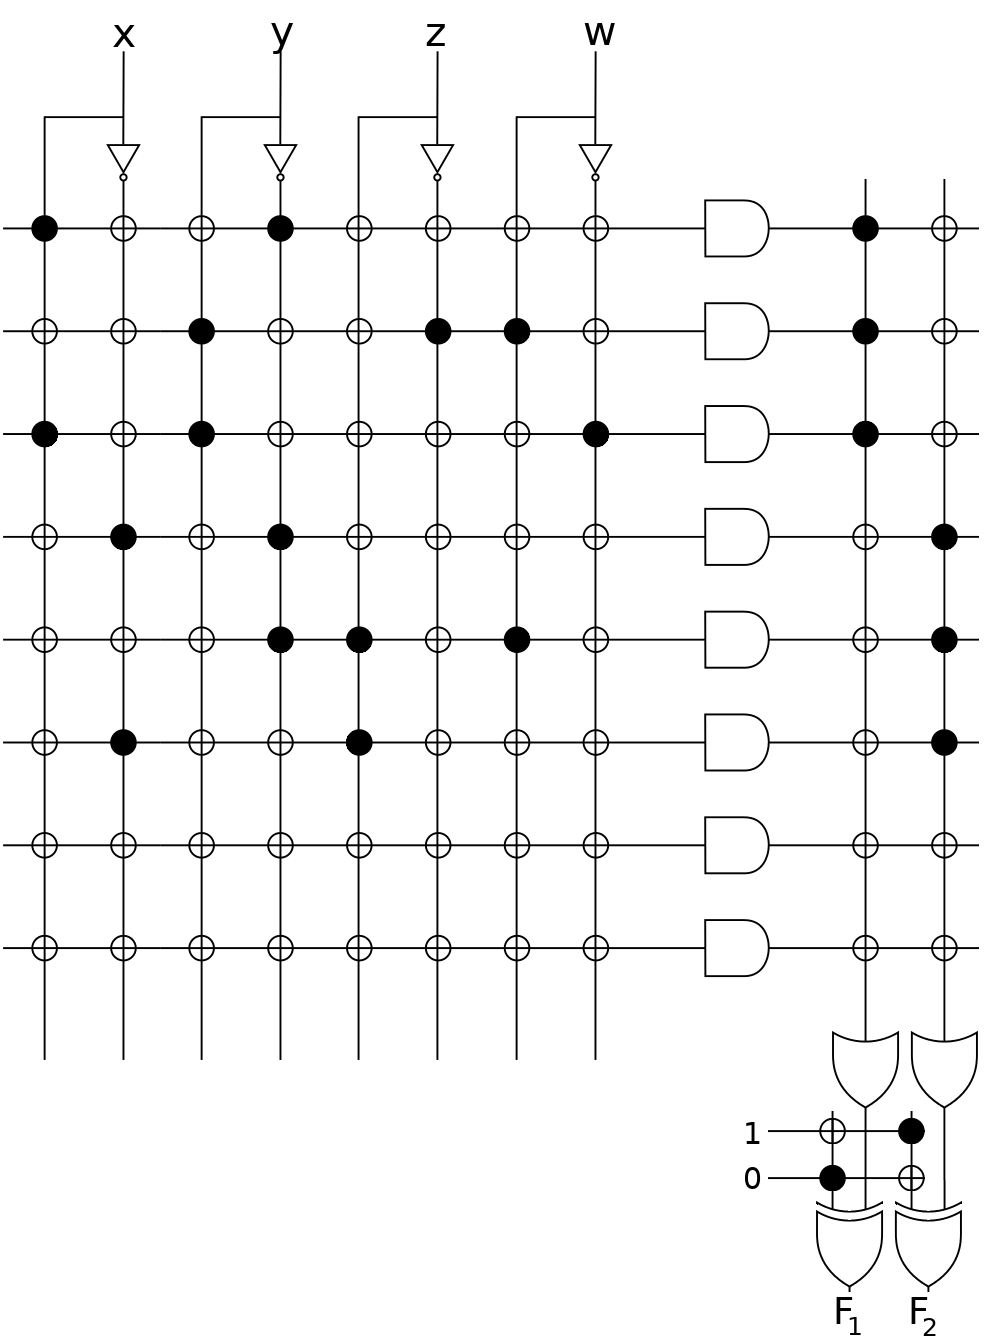
\includegraphics[width=\textwidth,height=\textheight,keepaspectratio]{PAL}
  \caption{PAL for $F_1$ og $F_2$\label{fig:PAL}}
\end{figure}
\clearpage

\section{Sekvensielle kretser}
Tidligere har vi forholdt oss til kombinatoriske kretser, der et sett med input
passerer gjennom én eller flere boolske funksjoner og blir output. En sekvensiell
krets har tilstand, som betyr at input til kretsen ikke bare kommer utenfra, men
også fra inni kretsen selv. Sannhetstabeller inneholder derfor nåværende tilstand
som input, og neste tilstand som output. Hvis man ikke er forsiktig kan dette gi
ustabile løkker, f.eks.\ en inverter som mater inn i seg selv og flyter mellom 0
og 1.

\subsection{Sekvensielle sannhetstabeller}
Sannhetstabellen til en sekvensiell krets kan ofte forenkles slik at man ikke
trenger å ha forrige output som input. Dette kan gjøres i tilfeller der neste
tilstand er uavhengig av forrige tilstand, eller i tilfeller der man med ord kan
beskrive hva som skjer med tilstanden. Se
Tabell~\ref{tab:sekvens-sannhet-vanskelig} og~\ref{tab:sekvens-sannhet-enkel}.

\begin{table}[hbt!]
  \centering
  \begin{minipage}{0.55\textwidth}
    \centering
    \begin{tabular}{cccc|cc}
      \toprule
      S & R & Q & $\bar{\text{Q}}$ & $\text{Q}_{next}$ & $\bar{\text{Q}}_{next}$ \\
      \midrule
      0 & 0 & 0 & 1 & 0 & 1 \\
      0 & 0 & 1 & 0 & 1 & 0 \\
      \midrule
      1 & 0 & 0 & 1 & 1 & 0 \\
      1 & 0 & 1 & 0 & 1 & 0 \\
      \bottomrule
    \end{tabular}
    \caption{Utdrag av sannehetstabell for SR-lås\label{tab:sekvens-sannhet-vanskelig}}
  \end{minipage}
  \begin{minipage}{.4\textwidth}
    \centering
    \begin{tabular}{cc|cc}
      \toprule
      S & R & Q & $\bar{\text{Q}}$  \\
      \midrule
      0 & 0 & \multicolumn{2}{c}{Uendret} \\
      \midrule
      1 & 0 & 1 & 0 \\
      \bottomrule
    \end{tabular}
    \captionof{table}{Forenklet versjon\label{tab:sekvens-sannhet-enkel}}
  \end{minipage}
\end{table}

\begin{center}
  \fbox{\begin{minipage}{.8\textwidth}
      \addtocontents{toc}{Låser vs. vipper}
    \textbf{Låser vs. vipper}\\
    Det later til å være variasjon i navnsetting av komponentene som følger. I
    dette dokumentet har jeg valgt å bruke \textit{lås} om alt som er
    nivåstyrt (eller ikke har noe styring), og \textit{vippe} om det som
    er flankestyrt. Dette er basert på diverse engelske definisjoner av
    henholdsvis \textit{latch} og \textit{flip-flop}.
  \end{minipage}}
\end{center}

\subsection{SR-lås}
En SR-lås er en sekvensiell krets bestående av to NOR-porter koblet i ``kryss''.
I tillegg kommer input $S$ og $R$ som står for \textit{Set} og \textit{Reset}.
Hver NOR-port har output ut av kretsen i tillegg til inn igjen i motsatt NOR\@.
Disse blir SR-låsens outputs, $Q$ og $\bar{Q}$. Se Figur~\ref{fig:SR-latch}.

\begin{figure}[hbt!]
  \centering
  \begin{minipage}{0.5\textwidth}
    \centering
    \begin{circuitikz} \draw
      (3,3) node[american nor port](R_NOR){}
      (3,0) node[american nor port](S_NOR){}

      (S_NOR.in 2) -- ++(-1,0) node[left]{$S$}
      (R_NOR.in 1) -- ++(-1,0) node[left]{$R$}

      (S_NOR.in 1) -- ++(-1,0) node[inner sep=0](S_IN){}
      (R_NOR.in 2) -- ++(-1,0) node[inner sep=0](R_IN){}

      (R_NOR.out) to[short,-*] ++(.5,0) node[inner sep=0](R_OUT){} -- ++(0,-.5) -- (S_IN)
      (S_NOR.out) to[short,-*] ++(.5,0) node[inner sep=0](S_OUT){} -- ++(0,.5)  -- (R_IN)

      (R_OUT) -- ++(1,0) node[right]{$Q$}
      (S_OUT) -- ++(1,0) node[right]{$\bar{Q}$}
      ;
    \end{circuitikz}
    \caption{Portdiagram for SR-lås \label{fig:SR-latch}}
  \end{minipage}\hfill
  \begin{minipage}{.45\textwidth}
    \centering
    \begin{tabular}{cc|cc}
      \toprule
      S & R & Q & $\bar{\text{Q}}$ \\
      \midrule
      0 & 0 & \multicolumn{2}{c}{Uendret} \\
      0 & 1 & 0 & 1 \\
      1 & 0 & 1 & 0 \\
      1 & 1 & \red{0} & \red{0} \\
      \bottomrule
    \end{tabular}
    \captionof{table}{Sannhetstabell for SR-lås\label{tab:SR-latch}}
  \end{minipage}
\end{figure}

SR-låsen fungerer ved at én av NOR-portene gir høy output, som får den andre til å
ha lav output. $Q$ og $\bar{Q}$ er altså motsatte under vanlig drift. Med $S$ og $R$
kan man styre hvilke NOR-porter som gjør hva. Når $S$ blir satt høy vil
NOR-porten til $\bar{Q}$ bli lav, som setter NOR-porten til $Q$ høy, som igjen går
inn i $\bar{Q}$ sin NOR-port og holder den lav. Motsatte skjer for $R$. Resultatet er
at en høy input på \textit{Set} setter $Q$ høy helt til \textit{Reset} blir satt
høy, som resetter $Q$ til lav. Se Tabell~\ref{tab:SR-latch}.

\textbf{Merk:} Før $S$ eller $R$ har vært høye er det umulig å vite tilstanden til bryteren.
Dersom både $S$ og $R$ er høye samtidig blir både $Q$ og $\bar{Q}$ $0$, og hvis begge
inputs går lave samtidig blir tilstanden igjen ubestemt.

\subsection{Eksitasjonstabell}
En eksitasjonstabell viser hvilke inputs som forursaker en ønsket
tilstandforandring. Venstresiden har nåværende og ønsket tilstand, og høyresiden
har hva input må være for å . Dersom en av inputenes tilstand ikke er vesentlig brukes $X$. For
et eksempel med SR-lås, se Tabell~\ref{tab:SR_latch_eksit}.

\begin{table}[hbt!]
  \centering
  \begin{tabular}{cc|cc}
    \toprule
    Q & Q$_{next}$ & S & R \\
    \midrule
    0 & 0 & 0 & X \\
    0 & 1 & 1 & 0 \\
    1 & 0 & 0 & 1 \\
    1 & 1 & X & 0
  \end{tabular}
  \caption{Eksitasjonstabell for SR-lås\label{tab:SR_latch_eksit}}
\end{table}

Det er verdt å merke at styring ofte ignoreres i eksitasjonstabeller, siden et
eventuelt \textit{enable}-signal uansett må være høyt for at en
tilstandsforanring skal kunne skje. Dette betyr at eksitasjonstabellen for en
SR-lås, en styrt SR-lås og en SR-vippe er identiske, selv om de har ulike
tilleggskrav til forandringer. 

\subsection{Styrt SR-lås}
En styrt SR-lås er en SR-lås der $S$ og $R$ kun har en virkning når en tredje
input $EN$ er høy. Dette ser man i blant annet en D-lås.

\subsection{D-lås}
En D-lås er en styrt SR-lås med kun én data-inngang $D$ og enable-inngangen
$EN$. SR-låsens input $S$ kommer fra $D$, og $R$ kommer
fra $\bar{D}$. Se Figur~\ref{fig:D-latch}.

\begin{figure}[hbt!]
  \centering
  \begin{circuitikz} \draw
    (3,3) node[american nor port](R_NOR){}
    (3,0) node[american nor port](S_NOR){}

    (S_NOR.in 2) -- ++(-1,0) node[american and port](S_AND){}
    (R_NOR.in 1) -- ++(-1,0) node[american and port](R_AND){}

    (S_NOR.in 1) -- ++(-1,0) node[inner sep=0](S_IN){}
    (R_NOR.in 2) -- ++(-1,0) node[inner sep=0](R_IN){}

    (R_NOR.out) to[short,-*] ++(.5,0) node[inner sep=0](R_OUT){} -- ++(0,-.5) -- (S_IN)
    (S_NOR.out) to[short,-*] ++(.5,0) node[inner sep=0](S_OUT){} -- ++(0,.5)  -- (R_IN)

    (R_OUT) -- ++(1,0) node[right]{$Q$}
    (S_OUT) -- ++(1,0) node[right]{$\bar{Q}$}

    (S_AND.in 1) -- ++(-.3,0) node[inner sep=0](S_EN){}
    (R_AND.in 2) -- ++(-.3,0) -- (S_EN) node[midway,inner sep=0](EN){}
    (EN) -- ++(-.8,0) node[left]{EN}

    (R_AND.in 1) node[above]{R} ++(-1,0) node[american not port](NOT){}
    (R_AND.in 1) ++(-2,0) coordinate(R_NOT_IN)
    (R_AND.in 1) -- (NOT.out)

    (S_AND.in 2) node[below]{S} -- ++(-2,0) node[circ](D){} -- (R_NOT_IN) -- (NOT.in)
    (D) -- ++(-1,0) node[left]{$D$}
    ;
  \end{circuitikz}
  \caption{Portdiagram for D-lås \label{fig:D-latch}}
\end{figure}

Når $EN$ er høy vil enten $S$ eller $R$ være høy, og SET/RESET-tilstanden blir
lagret. Når $EN$ blir lav vil tilstanden holdes, uavhengig av $D$.
En D-lås kan ses på som én bit med hukommelse, som husker hva $D$ var sist gang
$EN$ var høy. Se Tabell~\ref{tab:D-latch}.

\begin{table}[hbt!]
  \centering
  \begin{minipage}{.45\textwidth}
    \centering
    \begin{tabular}{ccc|c}
      \toprule
      D & EN & Q & Q$_{next}$\\
      \midrule
      X & 0 & 0 & 0 \\
      X & 0 & 1 & 1 \\
      1 & 1 & X & 1 \\
      0 & 1 & X & 0 \\
      \bottomrule
    \end{tabular}
    \caption{Sannhetstabell for D-lås\label{tab:D-latch}}
  \end{minipage}\hfill
  \begin{minipage}{.45\textwidth}
    \centering
    \begin{tabular}{cc|c}
      \toprule
      Q & Q$_{next}$ & D \\
      \midrule
      0 & 0 & 0 \\
      \midrule
      0 & 1 & 1 \\
      \midrule
      1 & 0 & 0 \\
      \midrule
      1 & 1 & 1 \\
      \bottomrule
    \end{tabular}
    \captionof{table}{Eksitasjonstabell for D-lås\label{tab:D-latch-eksit}}
  \end{minipage}
\end{table}

\section{Tidsdiagrammer}
TODO

\section{Klokkestyring}
Vi instroduserer et klokkesignal i kretsen for å kunne synkronisere dataflyt
mellom flere komponenter. Som oftest ser klokkesignalet ut som en firkantpuls
med 50\% høyt og 50\% lavt signal. Øyeblikket lav går til høy kalles stigende
flanke, og motsatt kalles synkedne flanke. Frekvensen blir antall stigende
flanker per sekund.

\subsection{Klokkestyrt D-lås}
En D-lås er allerede styrt med $EN$-inputen. For å gjøre den klokkestyrt kobler
man klokken til $EN$. Dette blir da en nivåstyrt lås, som henter inn data når
klokken er høy, og holder på dataen når klokken er lav.

\subsection{Oppsett- og holdetid}
$t_{setup}$ er tiden datasignalet må være stabilt før en endring i
klokkesignalet kan skje. $t_{hold}$ er tiden datasignalet må være stabilt etter
en endring i klokkesignal. Dette er fordi forsinkelser i porter gjør at
signalforandringer bruker en viss tid på å propagere ferdig. Hvis et annet
signal endres undeveis vil propageringen kunne skje kun delvis, og sluttilstanden
blir udefinert. For nivåstyrte kretser gjelder $t_{hold}$ fra nivået går ned.
For flankestyrte kretser er $t_{hold}$ tiden man må holde input etter
trigger-flanken.

\section{Flankestyring}
Forrige seksjon brukte klokkesignalet for å bestemme når data kunne endres, og
når data var låst fast. Dette kalles nivåstyring, siden nivåene på
klokkesignalet har betydning. I denne seksjonen er det ikke nivået som er
viktig, men øyeblikket nivået endres. Når klokke går fra lav til høy kaller vi
det stigende klokkeflanke (\rising), og motsatt høy til lav kalles synkende
klokkeflanke (\falling).
Vi opererer gjerne med at endringen skjer momentant, og at klokken er en perfekt
firkantbølge. Et flankestyrt komponent bryr seg ofte kun om én av flankene.

\subsection{Triggring}
Når et flankestyrt komponent mottar riktig flanke kaller vi det triggring. Da
hentes data inn fra input, og behandles av kretsen. Verdien på input er kun interresant i
trigger-øyeblikket, og frem til neste triggring vil kretsen være helt likegyldig
til input. Så lenge input er stabil i $t_{setup}$ før trigging, og $t_{hold}$
etter, kan input være hva enn den bare vil resten av tiden og ikke ha
noe å si.

I blokkdiagrammer har man et symbol for å vise at triggring skjer på stigende
klokkeflanke, se Figur~\ref{fig:SR-flip-flop-block}. Hvis triggring skjer på synkende
flanke vil klokkeinputen ha en sirkel foran seg, likt en pMOS\@.

\subsection{SR-vippe}
Aller først gjør vi en SR-lås til en SR-vippe, bare for å vise blokkdiagramformen,
sannhetstabellen, og timingdiagrammet. Se Figur~\ref{fig:SR-flip-flop-block} og Tabell~\ref{tab:SR-flip-flop-truth}.

\begin{figure}[hbt!]
  \centering
  \begin{minipage}{.45\textwidth}
    \centering
    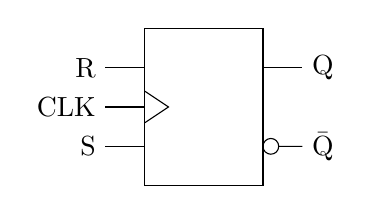
\begin{tikzpicture}
      \draw (0,0) rectangle (1.5,2);
      \draw (0,.8) -- (.3,1) -- (0,1.2);
      \draw (0,1) -- ++(-.5,0) node[left]{CLK};
      \draw (0,0.5) -- ++(-.5,0) node[left]{S};
      \draw (0,1.5) -- ++(-.5,0) node[left]{R};
      \draw (1.5,1.5) -- ++(.5,0) node[right]{Q};
      \draw (1.5,0.5) ++(.1,0) circle (.1) ++(.1,0) -- ++(.3,0) node[right]{$\bar{\text{Q}}$};
    \end{tikzpicture}
    \caption{Blokkdiagramform av SR-vippe\label{fig:SR-flip-flop-block}}
  \end{minipage}\hfill
  \begin{minipage}{.45\textwidth}
    \centering
    \begin{tabular}{ccc|cc}
      \toprule
      S & R & CLK & Q & $\bar{\text{Q}}$ \\
      \midrule
      0 & 0 & \rising{} & \multicolumn{2}{c}{Uendret} \\
      1 & 0 & \rising{} & 1 & 0 \\
      0 & 1 & \rising{} & 0 & 1 \\
      1 & 1 & \rising{} & \red{0} & \red{0} \\
      X & X & X & \multicolumn{2}{c}{Uendret} \\
      \bottomrule
    \end{tabular}
    \captionof{table}{Sannhetstabell for SR-vippe\label{tab:SR-flip-flop-truth}}
  \end{minipage}
\end{figure}

\subsection{D-vippe (Master-slave-vippe)}
To D-vipper i serie, der den éne mater den andre, men med omvendt klokkesignal. Se
figur~\ref{fig:master_slave}. Dette gjøres slik at å lese input $D$ og sende
output $Q$ er uavhengige. I vårt eksempel vil $D$ leses inn så lenge
klokken er lav, og i øyeblikket klokken går høy ``trigger'' vi vippen, og
signalet sendes ut $Q$. Endringer på $D$ vil ikke påvirke $Q$ før
neste triggring.

\begin{figure}[hbt!]
  \centering
  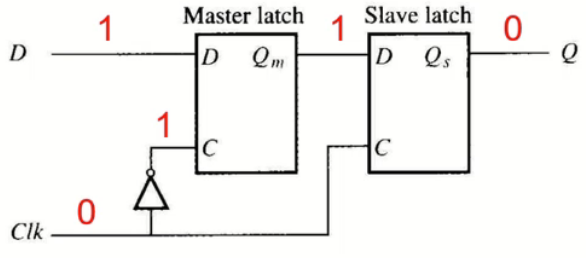
\includegraphics[width=0.7\textwidth,height=\textheight,keepaspectratio]{Krets_MasterSlave}
  \caption{D-vippe - to D-låser i master-slave-oppsett\label{fig:master_slave}}
\end{figure}

\begin{table}[hbt!]
  \centering
  \begin{tabular}{cc|cc}
    \toprule
    D & CLK & Q & $\bar{\text{Q}}$ \\
    \midrule
    0 & \rising{} & 0 & 1\\
    1 & \rising{} & 1 & 0\\
    X & X & \multicolumn{2}{c}{Uendret}\\
    \bottomrule
  \end{tabular}
  \caption{Sannhetstabell for D-vippe}
\end{table}

\subsection{Shift-register}
Ved å legge flere flankestyrte D-vipper i serie kan vi lage et shift-register der
flere bits er lagret i en slags kø, og kan shiftes bortover samtidig. Se Figur~\ref{fig:trigger_shift}.

\begin{figure}[hbt!]
  \centering
  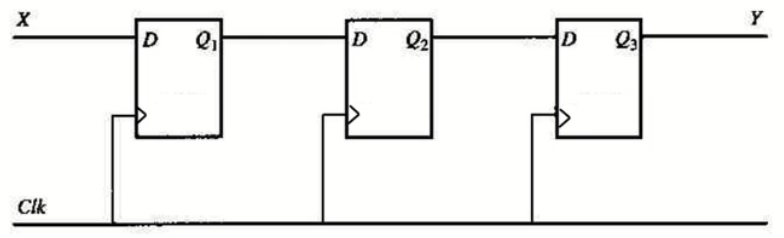
\includegraphics[width=0.7\textwidth,height=\textheight,keepaspectratio]{Krets_TriggerShift}
  \caption{Et shiftregister laget av flere master-slave-vipper i serie med samme trigger\label{fig:trigger_shift}}
\end{figure}

Hver av disse master-slave-vippene holder en verdi som de sender ut av hendholdsvis $Q_{1}$,
$Q_{2}$, $Q_{3}$. Ved stigende klokkeflanke vil hver vippe overskrives av det
den fikk inn i akkurat det øyeblikket. Resultatet er at køen går fremover.
Verdien i $Q_{3}$ forsvinner, og de andre verdiene rykker én plass frem. Verdien
$X$ stiller seg bakerst i køa.
\[
  Q_{3} \leftarrow Q_{2} \hspace{10mm} Q_{2} \leftarrow Q_{1} \hspace{10mm}  Q_{1} \leftarrow X
\]

\subsection{JK-vippe}
TODO
En JK-lås er en toggle

\subsection{T-vippe}
TODO
En T-lås er en toggle

\subsection{Registere}
TODO

\section{Databuss}
I digitale kretser der flere komponenter som skal kunne sende data til hverandre
er det upraktisk å ha koblinger mellom alle par. Derfor har man en felles
databuss, som alle komponentene kan bruke til å dele data. Tradisjonelt er
bussen mange parallelle ledninger. Buss-bredden er hvor mange bits som sendes i
parallell. Kun étt komponent kan sende data ut på bussen samtidig, så alle
komponentene har en kontroll-input som styrer skriving til bus. Dataen er trolig
også kun ment for ett annen komponent, så komponentene har også et
lesestyresignal. Alle komponentene er koblet på samme klokke, og på motsatte
flanker skrives og leses data fra bussen.

I en datamaskin med en CPU er det vanlig med tre busser, og CPUen er ``sjef''
for alle. Adresse-bussen styrer hvilken addresse i minne CPUen sikter til.
Data-bussen inneholder dataen som skal skrives til eller leses fra minne, og en
kontroll-bus holder kontroll på hvilke komponenter som skal lese og skrive.

Det finnes også serielle buser, der bits sendes i serie, f.eks. USB, som står
for Universal Serial Bus. Dette tillater faktisk raskere datastrømmer, siden
parallelle buser kan få problemer med ulik forplantningstid i ledningene, pluss
høyere induktans og kapasitans mellom ledningene.

\end{document}
